
En la figura~\figref{fig:fig_res_3} se muestra el gráfico de las soluciones del sistema del péndulo con los mismos parámetros que el segundo caso pedido, pero reduciendo el paso a $h = 0.001 \si[per-mode=symbol]{\second}$, se puede ver como se puede discernir mucho mejor la formas de las soluciones con esta mayor cantidad de puntos.\\
Finalmente en la figura~\figref{fig:fig_res_4} se puede ver las soluciones para el sistema para un caso en que no llegan casi a producirse oscilaciones, caso sobre-amortiguado, los parámetros para este caso son: 

\begin{equation*}
                \begin{array}{ll}
                  m = 1 \si[per-mode=symbol]{\kilo\gram} \\
                  l = 1 \si[per-mode=symbol]{\meter} \\  
                  b = 5 \si[per-mode=symbol]{\newton\second\per\meter} \\ 
                  h = 0.2 \si[per-mode=symbol]{\second} \\   
                  \Theta_{0} = 30 \si[per-mode=symbol]{\degree} \\  
                  \dot{\Theta}_{0} = 0 \si[per-mode=symbol]{\degree\per\second} \\            
                \end{array}
\end{equation*}




\clearpage


\begin{figure}[H] %htb
\begin{center}
\makebox[\textwidth]{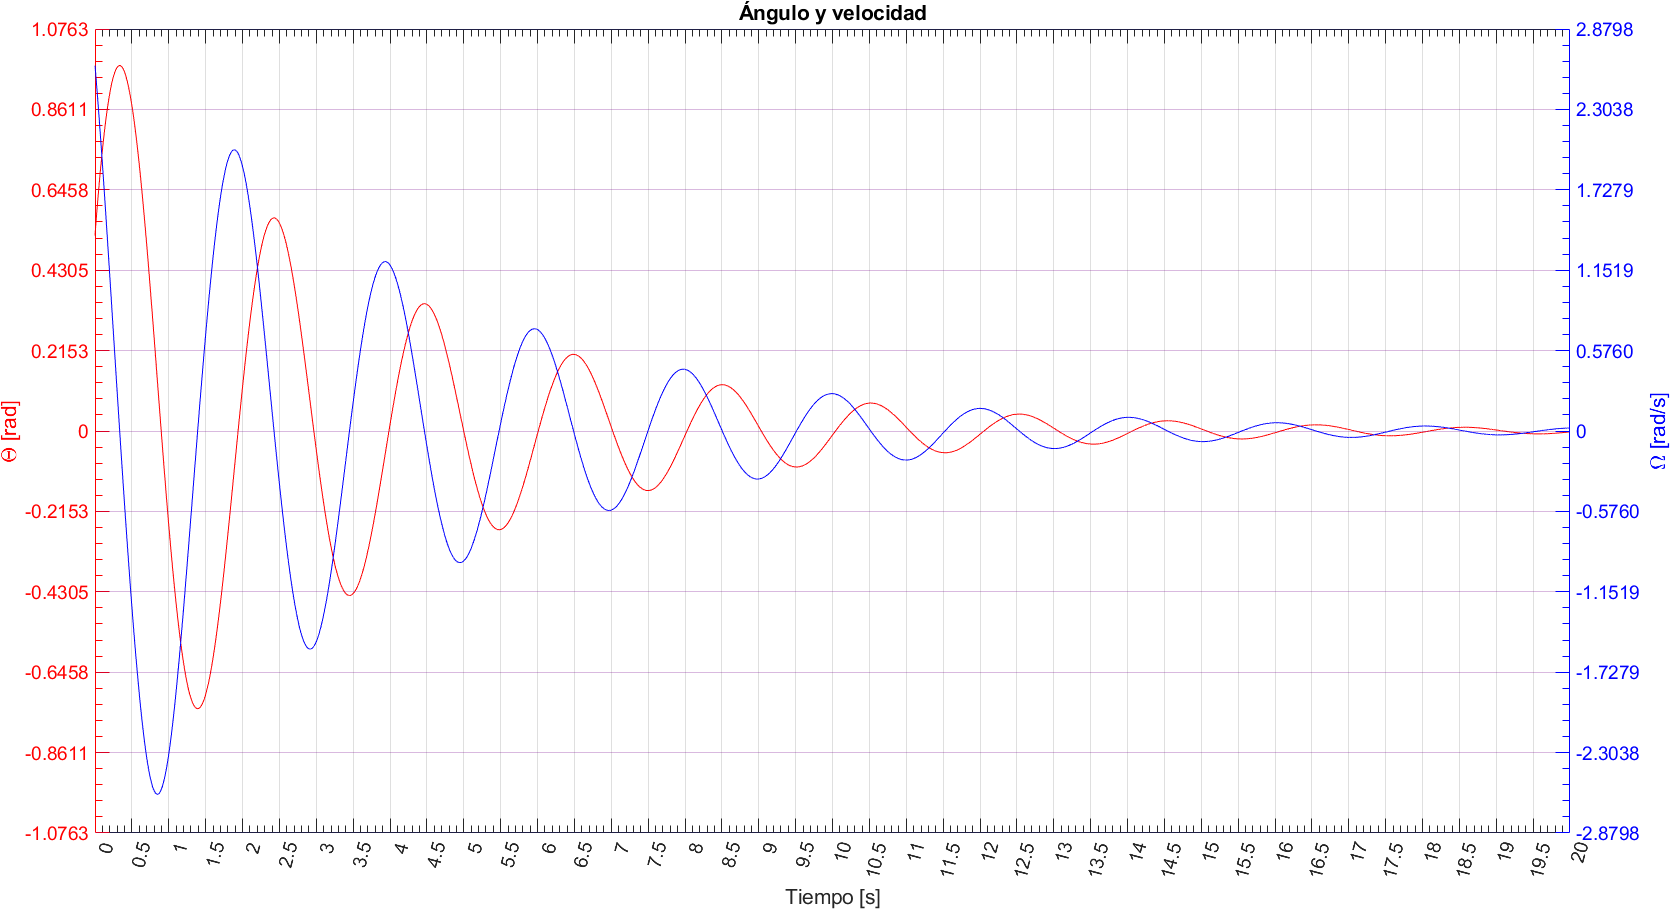
\includegraphics[width=0.95 \paperwidth,keepaspectratio=true, angle=90]{img/grafico_respuesta_3.png}} %% 
\caption{\label{fig:fig_res_3}\footnotesize{Gráfico de la solución para el primer caso con mayor cantidad de puntos.}}
\end{center}
\end{figure}

\clearpage


\begin{figure}[H] %htb
\begin{center}
\makebox[\textwidth]{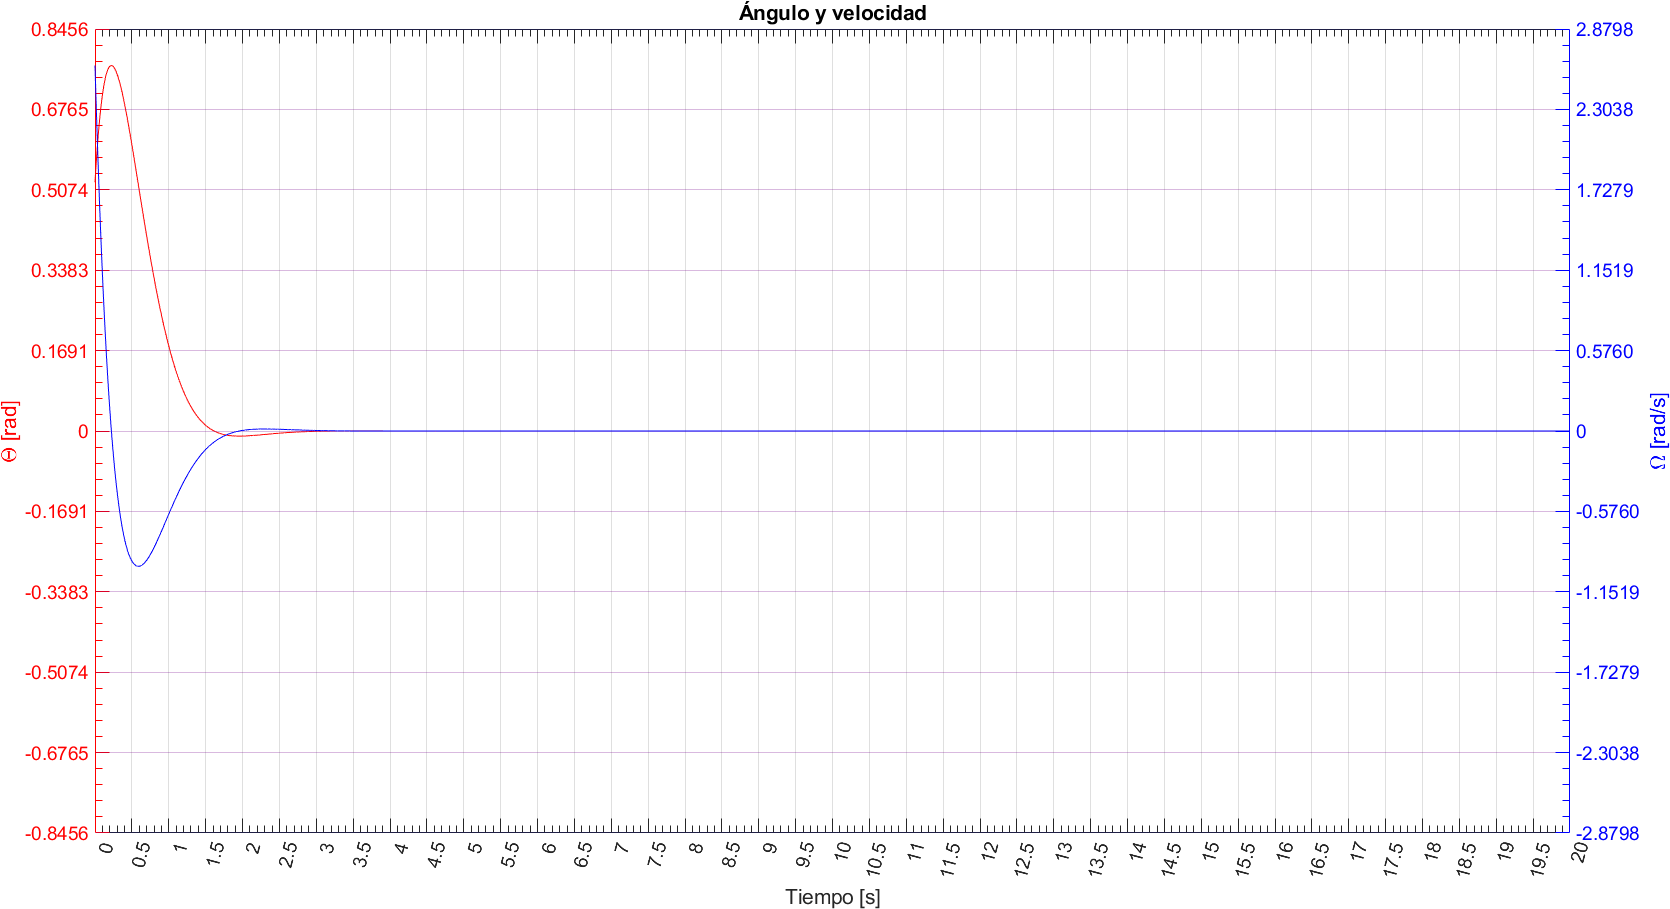
\includegraphics[width=0.95 \paperwidth,keepaspectratio=true, angle=90]{img/grafico_respuesta_4.png}} %% 
\caption{\label{fig:fig_res_4}\footnotesize{Gráfico de la solución para un sistema sobre-amortiguado.}}
\end{center}
\end{figure}
